\documentclass[12pt,a4paper]{scrartcl}
\usepackage[T2A, T1]{fontenc}
\usepackage[utf8]{inputenc}
\usepackage[english,russian]{babel}
\usepackage{misccorr}
\usepackage{graphicx}
\usepackage{amsmath}
\usepackage{amsfonts}
\usepackage{verbatim}
\usepackage{listings}
\usepackage{pgfplots}
\usepackage{graphicx}
\usepackage{pdfpages}
\DeclareUnicodeCharacter{03BB}{\ensuremath{\lambda}}
\DeclareUnicodeCharacter{03B7}{\ensuremath{\eta}}
\DeclareUnicodeCharacter{03C4}{\ensuremath{\tau}}
\DeclareUnicodeCharacter{03C1}{\ensuremath{\rho}}

\usepackage{algorithm}
\usepackage{algpseudocode}

% Настройки листингов.
\include{listings.inc}

\begin{document}
\begin{titlepage}
\newpage
\begin{center}
Федеральное государственное бюджетное образовательное учреждение  \\
\vspace{0.25cm}%расстояние до верхней строчки
высшего образования «Московский государственный технический  \\
\vspace{0.25cm}%расстояние до верхней строчки
университет имени Н.Э.Баумана (национальный исследовательский \\
\vspace{0.25cm}%расстояние до верхней строчки
университет)» (МГТУ им. Н.Э.Баумана) \\
%\hrulefill %горизонтальная черта
\end{center}
\vspace{5.0cm}
\begin{center}
\Large Отчёт по лабораторной работе №7 \\ По дисциплине «Анализ Алгоритмов» \\ Тема: «Муравьиный алгоритм» % \\ означает перенос
\end{center}
%\vspace{2.5em}
\vspace{6em}
\begin{flushright}
Студент: \hrulefill Шибанова Д.А. \\
\vspace{1.5em}
Группа: \hrulefill ИУ7-52\\
\vspace{1.5em}
Преподаватели: \hrulefill Волкова Л.Л., Строганов Ю.В.\\
\vspace{1.5em}
\end{flushright}
\vspace{\fill}
\begin{center}
Москва 2018
\end{center}
\end{titlepage}
\clearpage
\tableofcontents
\addcontentsline{toc}{section}{Введение}
\newpage
\begin{center}
Введение
\end{center}
Постановка задачи:

Реализовать алгоритм муравьиной колонии, решающий TSP задачу (задачу коммивояжёра). Необходимо найти кратчайший Гамильтонов цикл, т.е. цикл, который проходит все вершины, затрагивая каждую не более одного раза. Провести параметризацию алгоритма, т.е. подобрать такие параметры, при которых алгоритм лучше всего решает задачу, и исследовать зависимость работы алгоритма от регулирующих параметров. Провести сравнение с решением, найденным методом перебора.

Целью данной работы является изучение задачи коммивояжёра и способов её решения посредством алгоритмов природных вычислений.

Задачами данной работы является изучение муравьиного алгоритма, получение практических навыков его реализации, проведение сравнительного анализа поведения алгоритма при изменении его параметров, экспериментальное подтверждение различий алгоритма в зависимости от изменения параметров.

 \clearpage
\section{Аналитическая часть}

В данном разделе приводится теоретическое описание рассматриваемых в задаче алгоритмов.

\subsection{Описание алгоритмов} 

Задача коммивояжёра - одна из самых известных задач транспортной логистики. Одно из первых её решений было предложено У.Гамильтоном в XIX веке.
Суть задачи заключается в следующем:\\
необходимо найти оптимальный (кратчайший) путь через некоторые пункты, проходя каждый по одному разу. Мерой выгодности маршрута могут быть минимальное время, минимальные расходы на дорогу или минимальная длина пути. \cite{TSP}

В последние годы интенсивно развивается научное направление, называемое природными вычислениями, объединяющее математические методы, в основе которых заложены природные механизмы и принципы принятия решений, сформированные во флоре и фауне на протяжении миллионов лет. Имитация муравьиной колонии составляет основу муравьиных алгоритмов. Колония муравьёв рассматривается как многоагентная система, в которой каждый муравей рассматривается как отдельный агент, функционирующий автономно по простым правилам. \cite{AntAlg}

Классический муравьиный алгоритм - один из вариантов решения задачи коммивояжёра. Настоящие муравьи способны находить кратчайший путь между своим гнездом и источников пищи, используя не видимые глазу знаки, а с помощью информации из феромона. Когда муравей идёт, он оставляет на своей дороге феромон и ориентируется на путевые феромоны, оставленные другими муравьями. Если муравей подходит к точке выбора пути, где ни на одной дороге ещё нет феромона, то муравей выберет рандомно путь из возможных. Если путей в такой точке выбора было два, то половина муравьёв пойдёт налево, другая половина - направо. 

На рисунке \ref{graph2.1} представлен выбор путей муравьями при движении из двух вершин при отсутствии путевых феромонов других муравьёв. Красным обозначены точки выбора пути. 
\begin{figure}[h!]
	\centering
	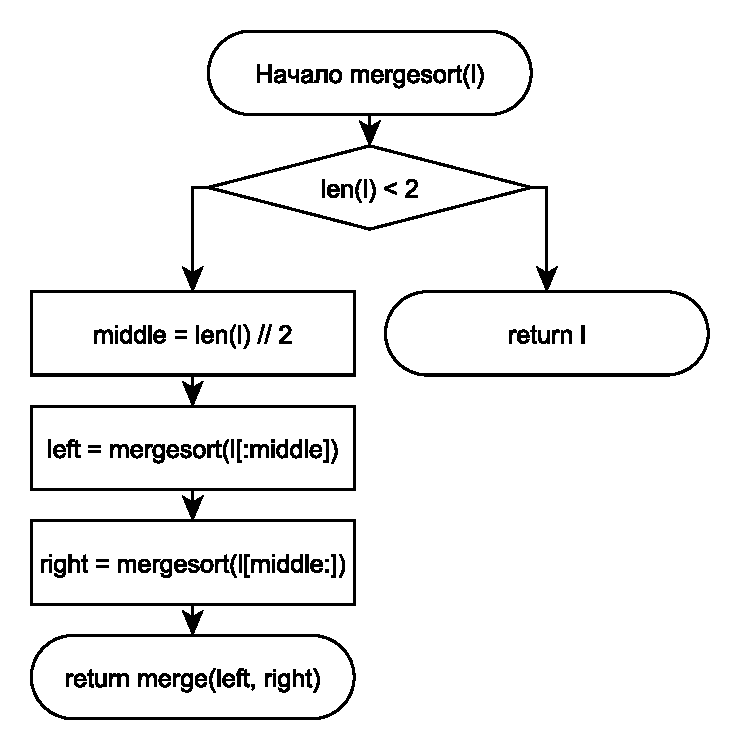
\includegraphics[width=\linewidth]{1.png}
	\caption{Выбор пути муравьём при отсутствии информации путевых феромонов}
	\label{graph2.1}
\end{figure}

Допустим, что исходно из каждой вершины вышло по 2 муравья. На рисунке \ref{graph2.2} показано, как распределятся муравьи по путям при отсутствии феромона.
\begin{figure}[h!]
	\centering
	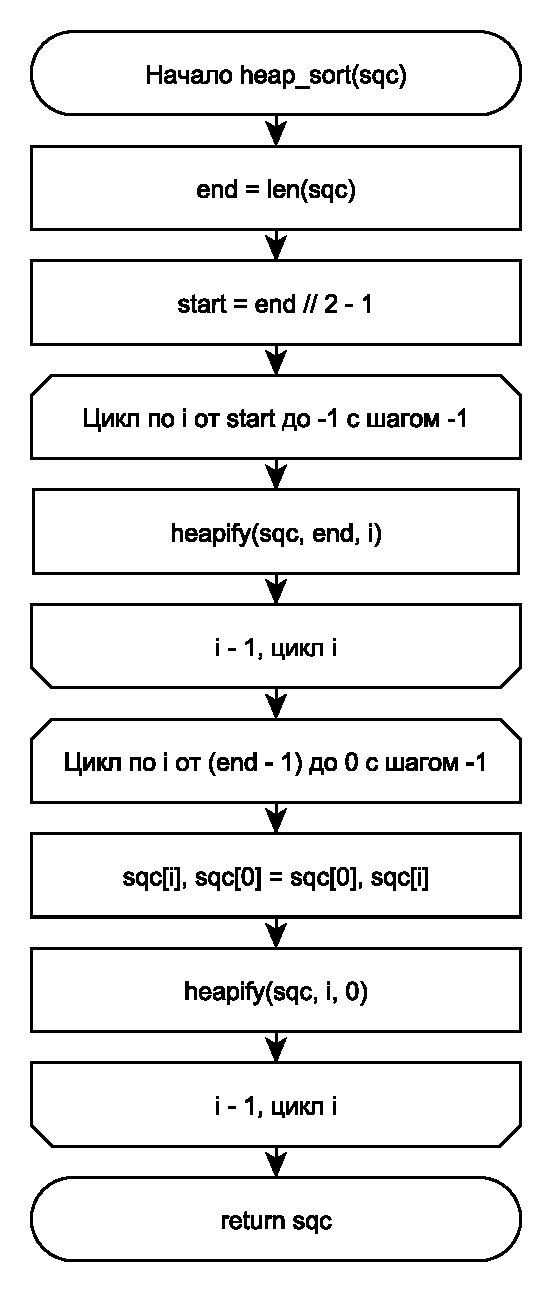
\includegraphics[width=\linewidth]{2.png}
	\caption{Выбор пути муравьём при отсутствии информации путевых феромонов}
	\label{graph2.2}
\end{figure}

Допустим, что все муравьи движутся примерно с одной скоростью. Если дороги были разной длины, то через некоторое время будет оставлено достаточно феромона, чтобы каждый муравей в точке выбора мог однозначно идентифицировать, какой путь был более популярен. 
Таким путём будет более короткий, поскольку муравьи будут проходить его быстрее, следовательно, будет оставлено больше феромона (рисунок \ref{graph2.3}). По мере роста количества феромона у более короткого пути уменьшается количество муравьёв, которые будут выбирать длинную дорогу. 
\begin{figure}[h!]
	\centering
	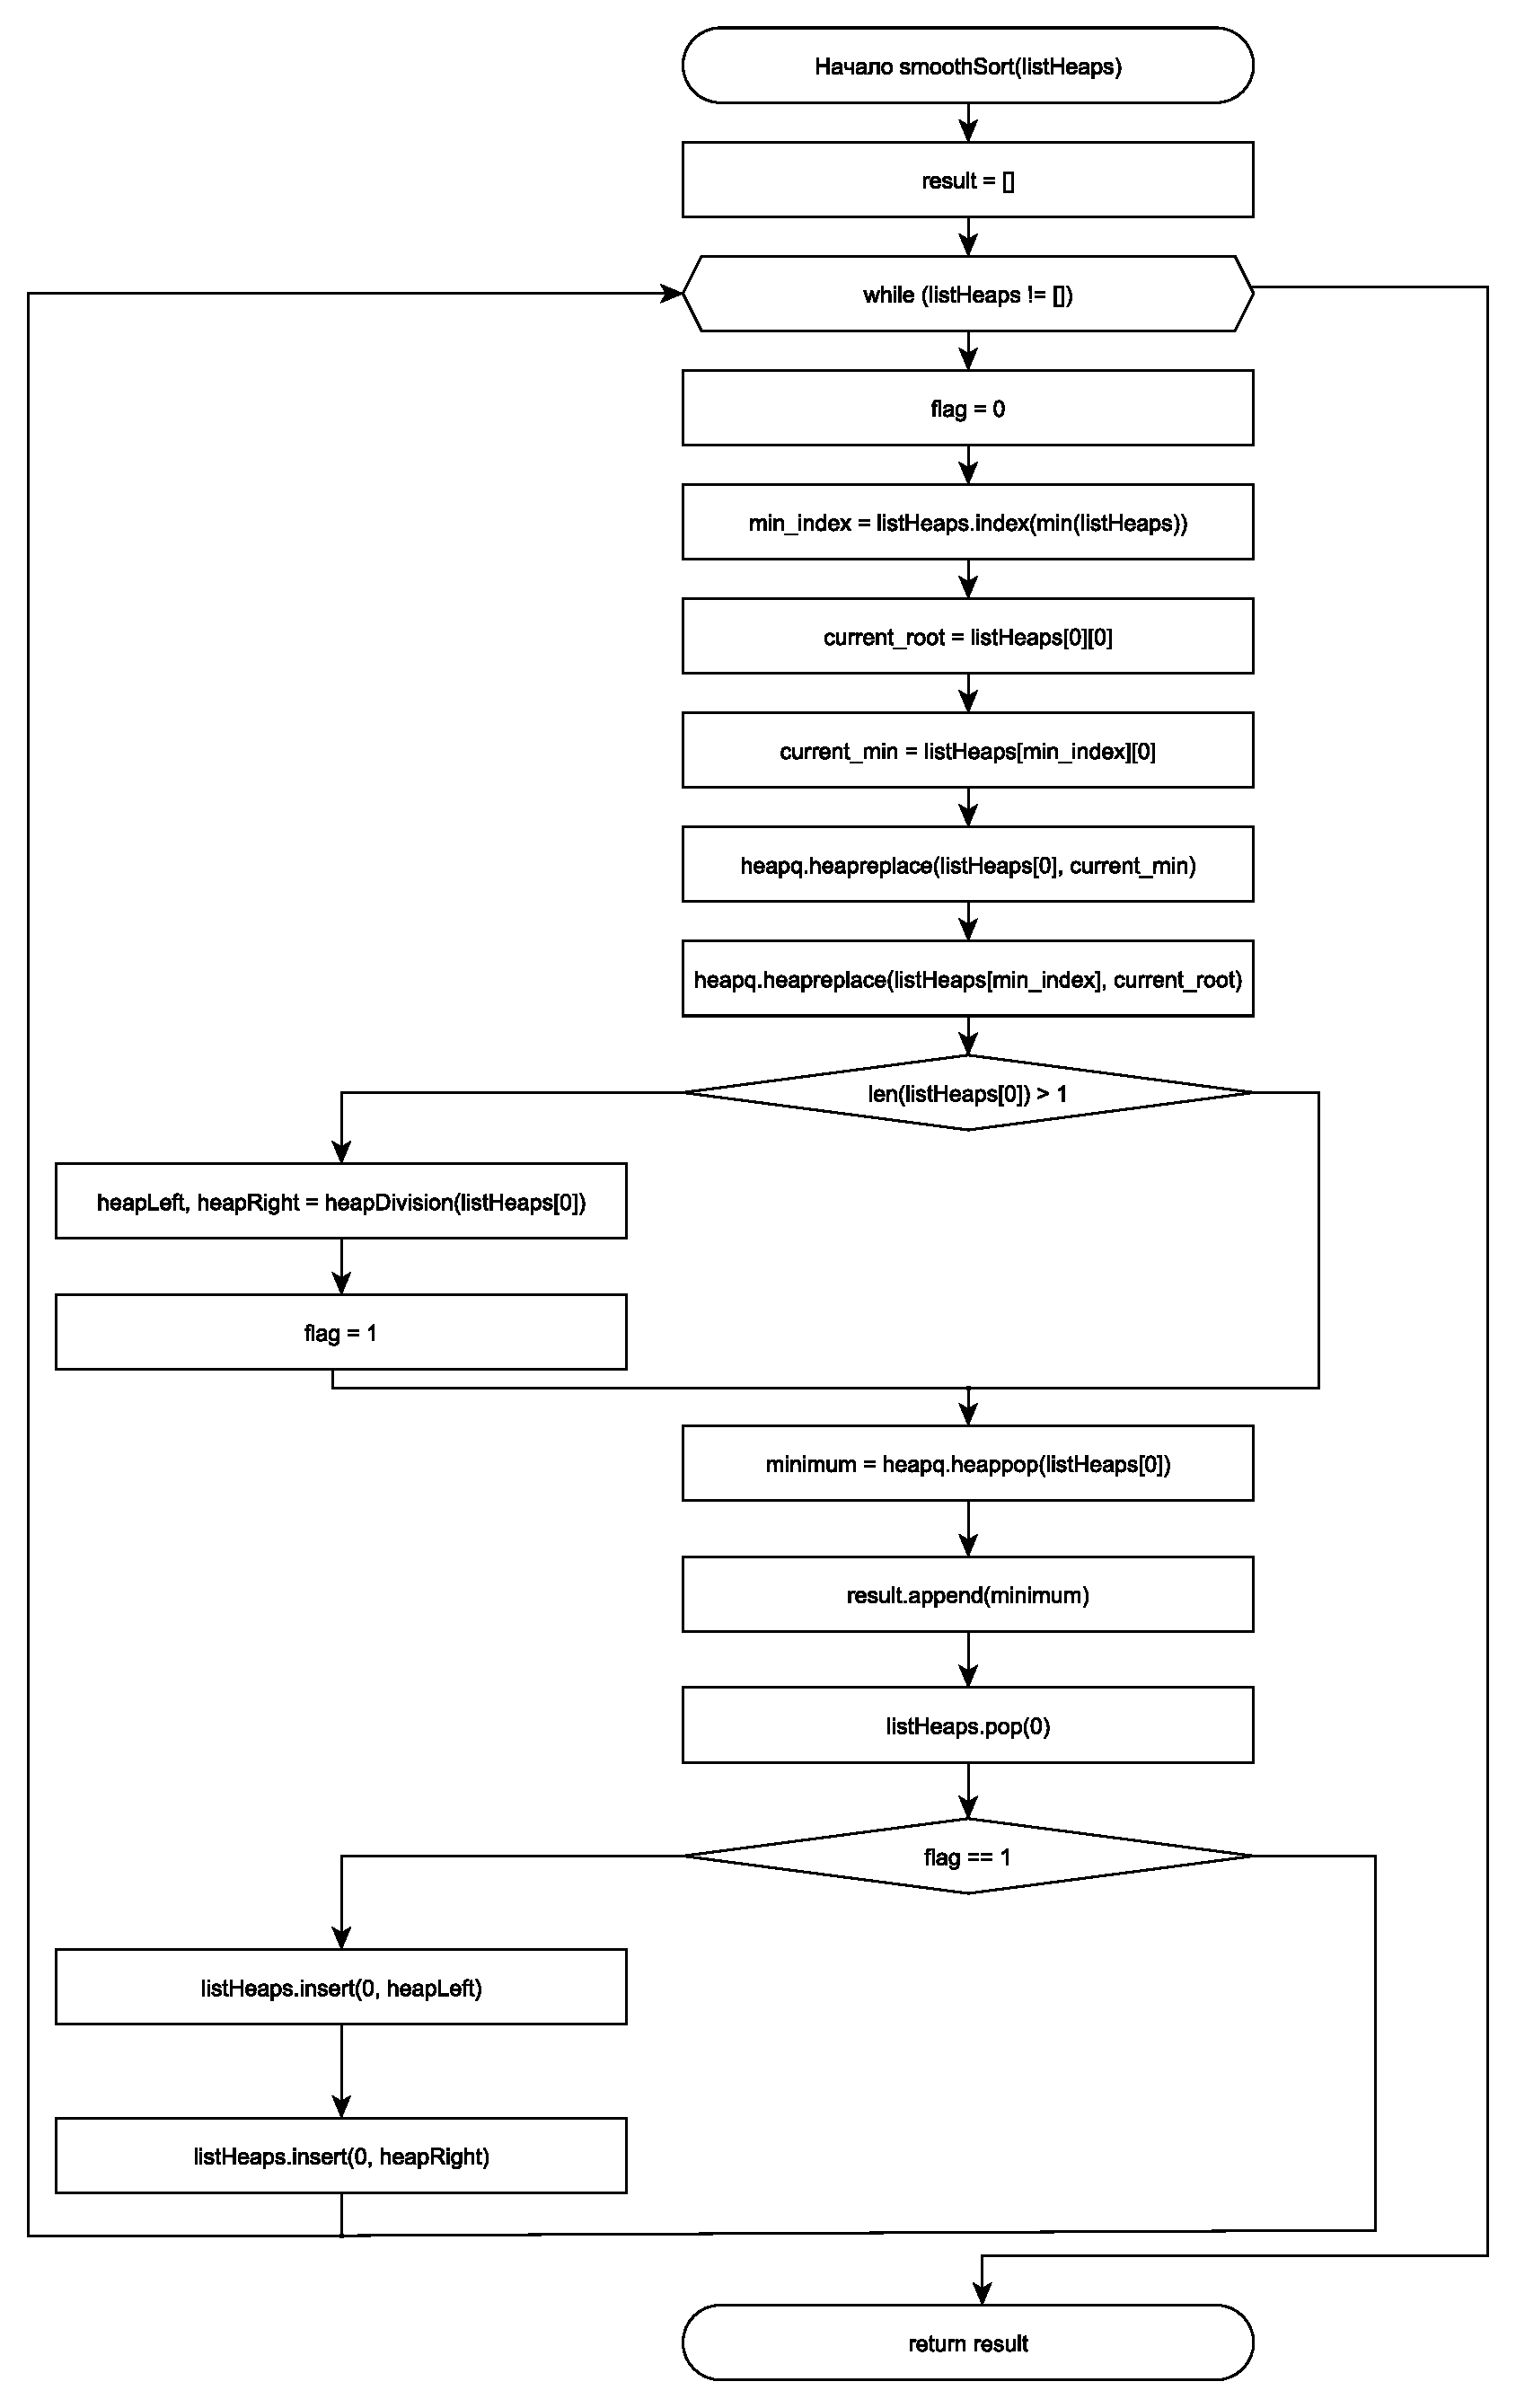
\includegraphics[width=\linewidth]{3.png}
	\caption{Выбор пути муравьём в результате обработки информации путевых феромонов}
	\label{graph2.3}
\end{figure}

Через некоторое время воздействие феромона у длинной дороги будет настолько низким, что все муравьи будут выбирать короткий путь.\cite{ACS}


Для описания поведения муравьёв в реальной жизни введена муравьиная система - алгоритм, в котором искусственно созданные "муравьи" совместно решают проблему обмена информацией через феромон при прохождении вершин графов. Основная идея данного генетического алгоритма состоит в следующем:
\begin{enumerate}
\item введём описание данных следующим образом:
\begin{enumerate}
\item существуют агенты, "муравьи";
\item каждый муравей обладает памятью - существует список городов 
\begin{equation}\label{eq2.1} 
J_{i,k}, 
\end{equation} 
которые нужно посетить k-ому муравью, если он находится в городе i;
\item каждый муравей обладает зрением - у муравья есть эвристическое желание посетить город j (находится он при этом в городе i) - это видимость 
\begin{equation}\label{eq2.2}
η_{ij} = \frac {1} {D_{ij}},
\end{equation}
где D - матрица расстояний (чем короче ребро, тем больше желание пройти по нему);
\item каждый муравей обладает обоняннием - муравей может улавливать феромон, оставленный другими муравьями;
\item происходит непрямой обмен - стигмерж - информацией между муравьями через окружающую среду;
\item муравей использует опыт колонии;
\item у колонии есть время жизни 
\begin{equation}\label{eq2.3}
1 \leqslant t \leqslant t_{max}
\end{equation}
\item на каждом шаге по времени все муравьи формируют по маршруту 
\begin{equation}\label{eq2.4}
T_k(t),
\end{equation}
длины маршрутов
\begin{equation}\label{eq2.5}
L_k(t)
\end{equation}
можно вычислить;
\end{enumerate}
\item в соответствии с длиной на рёбра маршрута накладывается феромон;
\item вместе с испарением феромона происходит переход на новый шаг по времени, при этом происходит обновление наилучшего маршрута
\begin{equation}\label{eq2.6}
T^*
\end{equation}
и длины наилучшего маршрута
\begin{equation}\label{eq2.7}
L^*
\end{equation}
в случае, если один из k муравьёв нашёл лучшее решение;
\item если муравей k находится в городе i, то переход в другой город j происходит по вероятностному правилу
\begin{equation}\label{eq2.8}
\begin{matrix}
P_{ij,k}(t) & = 
& \left\{
\begin{matrix}
0, & \mbox{ } j \notin J_{i,k} \\
\frac {(τ_{ij}(t))^\alpha * (η_{ij})^\beta} {\sum \limits_{q \in J_{i,k}} (τ_{iq}(t))^\alpha * (η_{iq})^\beta}, & \mbox{ } j \in J_{i,k}, \\
\end{matrix} \right.
\end{matrix}
\end{equation}
где τ - матрица значений феромона, $\alpha$ и $\beta$ - параметры, соблюдающие условие, что $\alpha + \beta = const$;
\item когда маршруты сформированы, каждый муравей оставляет на рёбрах своего маршрута $T_k(t)$ феромон
\begin{equation}\label{eq2.9}
\begin{matrix}
\Delta τ_{ij,k}(t) & = 
& \left\{
\begin{matrix}
0, & \mbox{ } (i, j) \notin T_k(t) \\
\frac {Q} {L_k(t)}, & \mbox{ } (i, j) \in T_k(t), \\
\end{matrix} \right.
\end{matrix}
\end{equation}
где Q - параметр того же порядка, что и $L^*$ - длина оптимального маршрута;
\item переход на следующий шаг по времени задействует ρ - коэффициент испарения феромона:
\begin{equation}\label{eq2.10}
τ_{ij}(t+1) = (1-ρ) * τ_{ij}(t) + \sum \limits_{k=1}^m \Delta τ_{ij,k}(t),
\end{equation}
где m - размер колонии.
\end{enumerate}
\cite{RECA}

В начале алгоритма количество феромона принимается равным небольшому положительному числу. Общее количество муравьёв остаётся постоянным и равным количеству городов, каждый муравей начинает маршрут из своего города. Данный генетический алгоритм можно модифицировать, введя $e$ элитных муравьёв, которые усиливают рёбра лучшего маршрута $T^*$:
\begin{equation}\label{eq2.11}
\Delta τ_{ij,e}(t) = \frac {e * Q} {L^*}
\end{equation} \cite{RECA}

Сложность алгоритма составляет $O(t_{max} \dot max(m,n^2))$, то есть сложность зависит от времени жизни колонии, количества городов и количества муравьёв в колонии. \cite{RECA}

\renewcommand{\listalgorithmname}{Список алгоритмов}
\floatname{algorithm}{Алгоритм}

Муравьиный алгоритм для задачи коммивояжёра: \\
%|1. Ввод матрицы расстояний D. \\
%|2. Инициализация параметров алгоритма. \\
%|3. Инициализация рёбер - присвоение видимости и начальной концентрации феромона. \\
%|4. Размещение муравьёв в случайно выбранные города без совпадений. \\
%|5. Выбор начального кратчайшего маршрута и определение длины лучшего текущего маршрута.\\
%|6. Цикл по времени жизни колонии t=1, $t_{max}$. \\
%|\quad6.1. Цикл по всем муравьям k=1,m. \\
%|\qquad6.1.1. Построить маршрут $T_k(t)$ по правилу \ref{eq2.8} и рассчитать длину $L_k(t)$. \\
%|\quad6.2. Конец цикла по муравьям. \\
%|\quad6.3. Проверка всех $L_k(t)$ на лучшее решение по сравнению с длиной лучшего текущего маршрута $L^*$. \\
%|\quad6.4. Если да, то обновить $L^*$ и $T^*$. \\
%|\quad6.5. Цикл по всем рёбрам графа. \\
%|\qquad6.5.1. Обновить следы феромона на ребре по правилам \ref{eq2.10} и \ref{eq2.11}. \\
%|\quad6.6. Конец цикла по рёбрам. \\
%|7. Конец цикла по времени. \\
%|8. Вывести кратчайший маршрут $T^*$ и его длину $L^*$.

\begin{algorithm}
\caption{Муравьиный алгоритм}\label{alg:Ants}
\begin{algorithmic}[1]
%\Comment{Под values обобщены непосредственные значения задаваемых параметров; под Parameters, соответсвенно, параметры}
 
 \State $D \gets \_values\_$
 \Comment{Ввод матрицы расстояний}
 
 \State $Parameters \gets \_values\_$
 \Comment{Инициализация параметров алгоритма}
 
 \State $Feromon \gets \_values\_$
  \Comment{Инициализация начальной концентрации феромона}
 \State $η_{ij} \gets \_values\_$
 \Comment{Инициализация видимости}
 
 \State $T^* \gets \_values\_$
 \State $L^* \gets \_values\_$
 \Comment{Выбор начального текущего маршрута и определение длины лучшего текущего маршрута}
 
 \For{t=1;  $t_{max}$; t++}
 \Comment{Цикл по времени жизни колонии}
 \For{k=1; m; k++}
 \Comment{Цикл по всем муравьям}
\State Построить маршрут $T_k(t)$ по правилу \ref{eq2.8} и рассчитать длину $L_k(t)$.
\EndFor
\If { $L_k(t)$ < $L^*$}
\Comment{Если найден лучший путь}
\State Обновить $L^*$ и $T^*$
\EndIf
\For{рёбра графа}
\State{Обновить следы феромона на ребре по правилам \ref{eq2.10} и \ref{eq2.11}}
\EndFor
\EndFor

\State Print($T^*$ и $L^*$) 
\Comment{Вывести кратчайший маршрут $T^*$ и его длину $L^*$}
 
\end{algorithmic}
\end{algorithm}
 
%\listofalgorithms

 \clearpage
\section{Конструкторская часть}

В данном разделе приводятся описания алгоритмов и блок-схемы их работы.

\subsection{Разработка алгоритмов}

Блок-схемы алгоритмов

На схеме \ref{graph2.4} представлена работа алгоритма нахождения решения задачи коммивояжёра перебором.

\begin{figure}[h!]
	\centering
	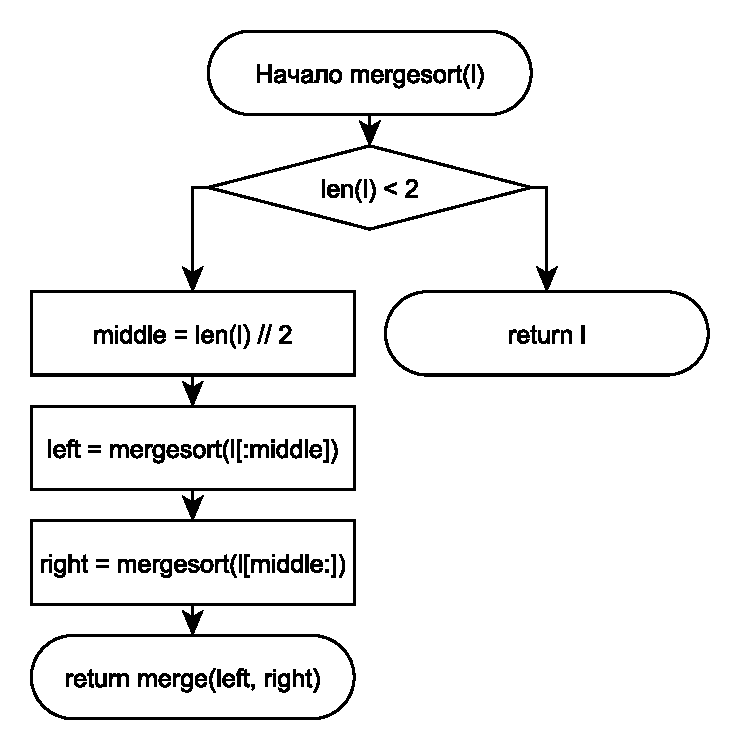
\includegraphics[width=\linewidth]{1.pdf}
	\caption{Нахождение решения перебором}
	\label{graph2.4}
\end{figure}

На схеме \ref{graph2.5} представлен муравьиный алгоритм для решения задачи коммивояжёра.

\begin{figure}[h!]
	\centering
	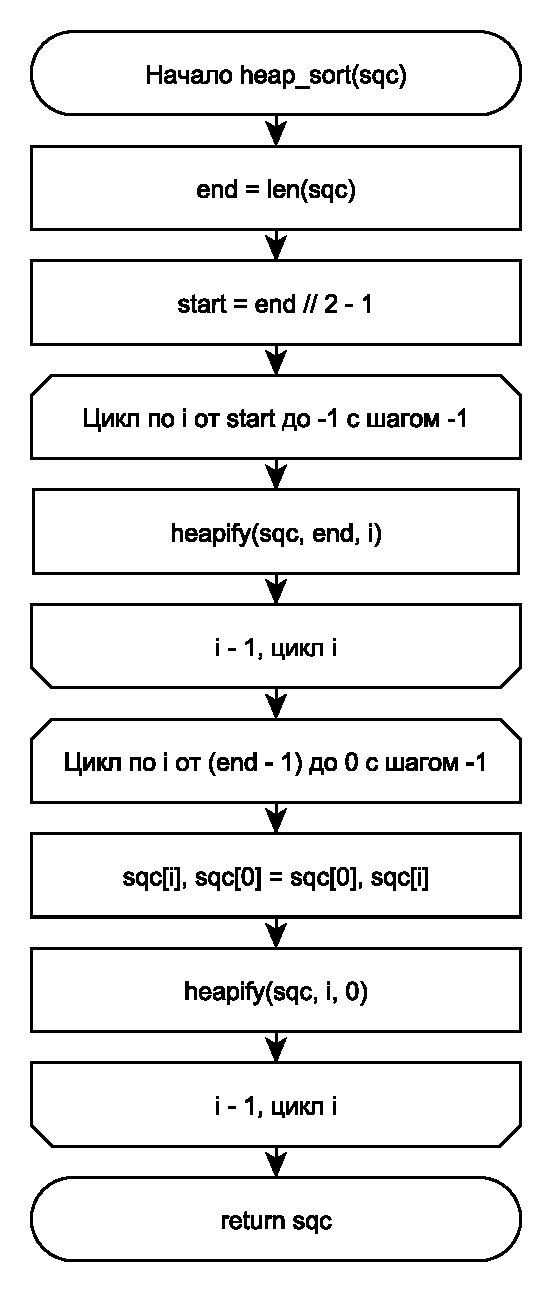
\includegraphics[width=\linewidth]{2.pdf}
	\caption{Муравьиный алгоритм}
	\label{graph2.5}
\end{figure}

\subsection{Исследование зависимости поведения алгоритма от изменяемых параметров}

Рассмотрим формулу
\begin{equation*}
\begin{matrix}
P_{ij,k}(t) & = 
& \left\{
\begin{matrix}
0, & \mbox{ } j \notin J_{i,k} \\
\frac {(τ_{ij}(t))^\alpha * (η_{ij})^\beta} {\sum \limits_{q \in J_{i,k}} (τ_{iq}(t))^\alpha * (η_{iq})^\beta}, & \mbox{ } j \in J_{i,k}. \\
\end{matrix} \right.
\end{matrix}
\end{equation*}

Её результатом будет являться вероятность, которая не будет превышать значение, равное единице. Обеспечивается это тем, что внизу стоит сумма произведений для всех граней, а сверху - только для одной, входящей в сумму знаменателя.

Как было указано в аналитическом разделе, формула обладает двумя регулируемыми параметрами:\\
$\alpha$ - значимость для муравья феромона, оставленного на путях; \\
$\beta$ - важность расстояния до конкретного города.\\
Если отрегулировать данные параметры, можно добиться разной эффективности работы алгоритма. 

В частности, если, к примеру, $\alpha = 0$, то алгоритм из муравьиного вырождается в жадный алгоритм, то есть муравей игнорирует опыт предыдущих агентов и просто выбирает самое кратчайшее ребро из всех возможных. Минусом такого выбора может являться то, что нет гарантии, что такой путь даст наилучшее решение, поскольку у более длинного ребра дальнейший путь может оказаться короче, чем тот, который получится по сделанному муравьём выбору.

Если же принять $\beta = 0$, то муравей игнорирует расстояние и руководствуется лишь феромоном, оставленным на путях. В таком случае алгоритм не зависит от конкретного расположения городов вообще, то есть характер его работы случайный, а результат непредсказуемый, что может дать в конкретных ситуациях такое решение, которое окажется хуже результата в случае превращения алгоритма в жадный.

Важно понимать, что нельзя слишком большую роль отводить случайности, а именно это и регулирует параметр $\beta$. Случайность в алгоритме должна лишь давать шанс на то, что будет выбран не самый оптимальный на первый взгляд путь, который может быть самым кратчайшим в дальнейшей перспективе.

Из данных соображений можно сделать вывод, что необходимо всегда устанавливать более значимым параметр $\beta$, однако М.Дориго, автор алгоритма, утверждает, что наилучший результат достигается при $\alpha = \beta$.

На феромон оказывает влияние параметр ρ - коэффициент испарения феромона:
\begin{equation*}
τ_{ij}(t+1) = (1-ρ) * τ_{ij}(t) + \sum \limits_{k=1}^m \Delta τ_{ij,k}(t).
\end{equation*}

Если $ρ = 0$, то феромон не испаряется вообще. Построим рассуждения следующим образом:
\begin{enumerate}
\item в самом начале количество феромона везде одинаково, вероятнее всего то, что муравей пойдёт к самому ближайшему городу; 
\item так как феромон не испарялся, перевес ближайшего города начинает увеличиваться;
\item как итог, все муравьи будут выбирать кратчайшее ребро из доступных, следовательно, будет получена версия жадного алгоритма.
\end{enumerate}

Если $ρ = 1$, то испаряется весь феромон, а это значит, что роль предыдущих поколений сводится к нулю. Теряется сам смысл муравьиного алгоритма - опора на опыт предыдущих агентов.

В результате, можно прийти к выводу, что испарение не должно принимать крайних значений, находясь между ними. Вероятно, оптимальным значением может быть $ρ \approx 0.5$, которое может несколько увеличиваться или уменьшаться, но при большом отклонении значения к крайним есть потенциальная вероятность вырождения алгоритма в жадный или вероятность потери опоры на опыт других поколений.

 \clearpage
\section{Технологическая часть}

В данном разделе приводятся средства реализации и листинг кода.

\subsection{Требования к программному обеспечению}

Минимальные системные требования: PC с операционной системой Windows версии XP/Vista/7/8/10. Требуются устройства ввода: клавиатура, мышь. 

\subsection{Средства реализации}

Для выполнения работы был выбран язык программирования Python ввиду его простоты.

\subsection{Листинг кода}   

Решение перебором:
%\begin{lstlisting}[label=some-code,caption=Перебор]
%\end{lstlisting}
\begin{verbatim}
# поиск в глубину полного маршрута
def look_throught(arr, pos, visited, dist=0):
    if len(visited) == len(arr):
        #print(visited, dist)
        return visited, dist

    min_dist = -1
    min_path = []
    for j in range(0, len(arr)):
        if arr[pos][j] > 0 and j not in visited:
            buf = [j]
            buf.extend(visited)
            new_visited, new_dist = \
                      look_throught(arr, j, buf, dist + arr[pos][j])
            if new_dist != -1 and (min_dist > new_dist or min_dist == -1):
                min_dist = new_dist
                min_path = new_visited

    return min_path, min_dist

# нахождение решения перебором
def stupid_solver(arr):
    min_dist = -1
    min_path = []
    for i in range(0, len(arr)):
        new_visited, new_dist = look_throught(arr, i, [i])
        if new_dist != -1 and (min_dist > new_dist or min_dist == -1):
            min_dist = new_dist
            min_path = new_visited

    min_path.reverse()
    return min_path, min_dist
\end{verbatim}

Муравьиный алгоритм:
%\begin{lstlisting}[label=some-code,caption=Муравьиный алгоритм]
%\end{lstlisting}
\begin{verbatim}
# нахождение решения муравьиным алгоритмом
def ant_solver(arr, start_f, alpha, beta, ro, lifetime, Q):
    feromon = [[start_f for j in range(len(arr))] for i in range(len(arr))]

    for time in range(lifetime):
        #print(feromon) # состояние феромонов
        new_path = [] # маршрут для каждого муравья
        new_len = [] # длина пути каждого муравья

        # ищем новый маршрут муравья
        for ant in range(len(arr)):
            new_path.append([ant])
            new_len.append(0)
            
            while True:
                # куда можно послать муравья
                where_to_go = []
                for i in range(len(arr)):
                    if i not in new_path[ant] and arr[new_path[ant][-1]][i] > 0:
                        where_to_go.append(i)
                # муравей больше не может идти в этом направлении
                if len(where_to_go) == 0:
                    break
                # куда мы пошлём муравья
                sum_variants = 0
                
                for variant in where_to_go:
                    sum_variants += (feromon[new_path[ant][-1]] \ 
                    [variant] ** alpha) * \
                    ((1 / arr[new_path[ant][-1]] \ 
                    [variant]) ** beta)

                choice = random()
                choice_var = 0
                while choice > 0:
                    choice -= (feromon[new_path[ant][-1]] \ 
                        [where_to_go[choice_var]] ** alpha) * \
                        ((1 / arr[new_path[ant][-1]]
                        [where_to_go[choice_var]]) ** beta) / sum_variants
                    choice_var += 1
                    if choice_var == len(where_to_go):
                        choice_var -= 1
                        break

                new_len[ant] += arr[new_path[ant][-1]][where_to_go[choice_var]]
                new_path[ant].append(where_to_go[choice_var])                        

        # феромон испарился
        for i in range(len(feromon)):
            for j in range(len(feromon)):
                feromon[i][j] *= (1 - ro)

        # муравьи "докинули" феромон
        for i, ant_path in enumerate(new_path):
            for i in range(1, len(ant_path)):
                #feromon[ant_path[i-1]][ant_path[i]] += Q / new_len[i]
                feromon[ant_path[i-1]][ant_path[i]] += Q / new_len[i] * \
                    len(ant_path) / len(arr)
                
        # значение не должно быть ниже минимального
        for i in range(len(feromon)):
            for j in range(len(feromon)):
                feromon[i][j] = max(feromon[i][j], start_f)

    min_len = -1
    min_path = []
    for i, l in enumerate(new_len):
        if len(new_path[i]) == len(arr):
            if min_len == -1 or l < min_len:
                min_len = l
                min_path = new_path[i]

    return min_path, min_len
\end{verbatim}


 \clearpage
\section{Экспериментальная часть}

В данном разделе приводится пример работы алгоритма, происходит экспериментальное сравнение параметров, используемых в алгоритме.

\subsection{Примеры работы}

Для тестирования и оценки параметров был выбран граф, представленный на рисунке \ref{graph2.6} и заданный следующей матрицей (первая строка и первый столбец задают города, пересечения их элементов задают расстояние между городами, если между ними есть прямой путь):

\begin{figure}[h!]
	\centering
	\includegraphics[width=\linewidth]{4.png}
	\caption{Граф, на котором проводилось тестирование}
	\label{graph2.6}
\end{figure}

\begin{table}[ht]
	\caption{Матрица расстояний между городами}
	\begin{tabular}{|l|c|c|c|c|c|}
		\hline
		 & Г1 & Г2 & Г3 & Г4 & Г5\\
		\hline
		\hline
		Г1 & 0 & 5 & 2  & 7 &  0\\
		\hline
		Г2 & 5 & 0 & 4 & 0 & 9\\
		\hline
		Г3 & 2 & 4 & 0 & 4 & 10\\
		\hline
		Г4 & 7 & 0 & 4 & 0 & 4\\
		\hline
		Г5 & 0 & 9 & 10 & 4 & 0\\
		\hline
	\end{tabular}
	\label{tab:tabular}
\end{table}

Для данной матрицы лучший путь, обнаруженный муравьиной колонией, составлял 17. \\

Нахождение решение перебором обнаружило результат, равный 15. 

Сравнение времени работы алгоритмов при различном времени жизни колонии: 

\begin{table}[ht]
	\caption{Время работы алгоритмов}
	\begin{tabular}{|l|c|c|c|}
		\hline
		Время жизни колонии & Перебор & Муравьи & Разница времени работы в процентах\\
		\hline
		\hline
		1 & 0.000223 & 0.000168 & -33\%\\
		\hline
		10 & 0.000249 & 0.001213 & +21\%\\
		\hline
		100 & 0.000282 & 0.012529 & +98\%\\
		\hline
		1000 & 0.000238 & 0.127736 & +193\%\\
		\hline
		10000 & 0.000222 & 1.216264 & +292\%\\
		\hline
	\end{tabular}
	\label{tab:tabular}
\end{table}

\subsection{Постановка эксперимента}  

На графике \ref{graph4.1} представлена зависимость средних значений длины пути при времени жихни колонии на выборках от 1 до $10^4$ от параметров $\alpha$ и ρ (параметр $\beta$ связан со значением $\alpha$, поэтому на графике не рассматривается отдельно).

\pgfplotsset{compat=1.9}
\pgfplotsset{Param/.style = {blue, samples = 100}}
\begin{figure}
	\begin{tikzpicture}
	\begin{axis}[zlabel=Средняя длина пути, ylabel=ρ, xlabel=$\alpha$, width = 15cm, xmin = 0, ymin = 0, legend pos = north west]
	\legend{Зависимость от параметров}
	\addplot3[Param] table {
		x            y            z
		0           0            19.2
		0           0.2         17.4
		0           0.4         17.0
		0           0.6         18.6
		0           0.8         18.6
		0           1            17.8
		0.2        0            18.4
		0.2        0.2         18.0
		0.2        0.4         18.0
		0.2        0.6         17.4
		0.2        0.8         20.0
		0.2        1            18.2
		0.4        0            18.0
		0.4        0.2         18.6
		0.4        0.4         17.8
		0.4        0.6         19.0
		0.4        0.8         18.6
		0.4        1            18.2
		0.6        0            18.2
		0.6        0.2         20.2
		0.6        0.4         17.4
		0.6        0.6         18.4
		0.6        0.8         19.0
		0.6        1            19.2
		0.8        0            18.2
		0.8        0.2         18.6
		0.8        0.4         18.6
		0.8        0.6         18.2
		0.8        0.8         17.4
		0.8        1           17.4
		1           0           17.8
		1           0.2        18.0
		1           0.4        18.2
		1           0.6        17.8
		1           0.8        17.0
		1           1           17.8
	};
	\end{axis}
	\end{tikzpicture}
	\caption{График зависимостей параметров $\alpha$, ρ и среднего значения найденного пути за всё время жизни колонии при данных параметрах}
	\label{graph4.1}
\end{figure}

На рисунке \ref{graph2.7} представлены средние значения с помощью поверхностной диаграммы.

\begin{figure}[h!]
	\centering
	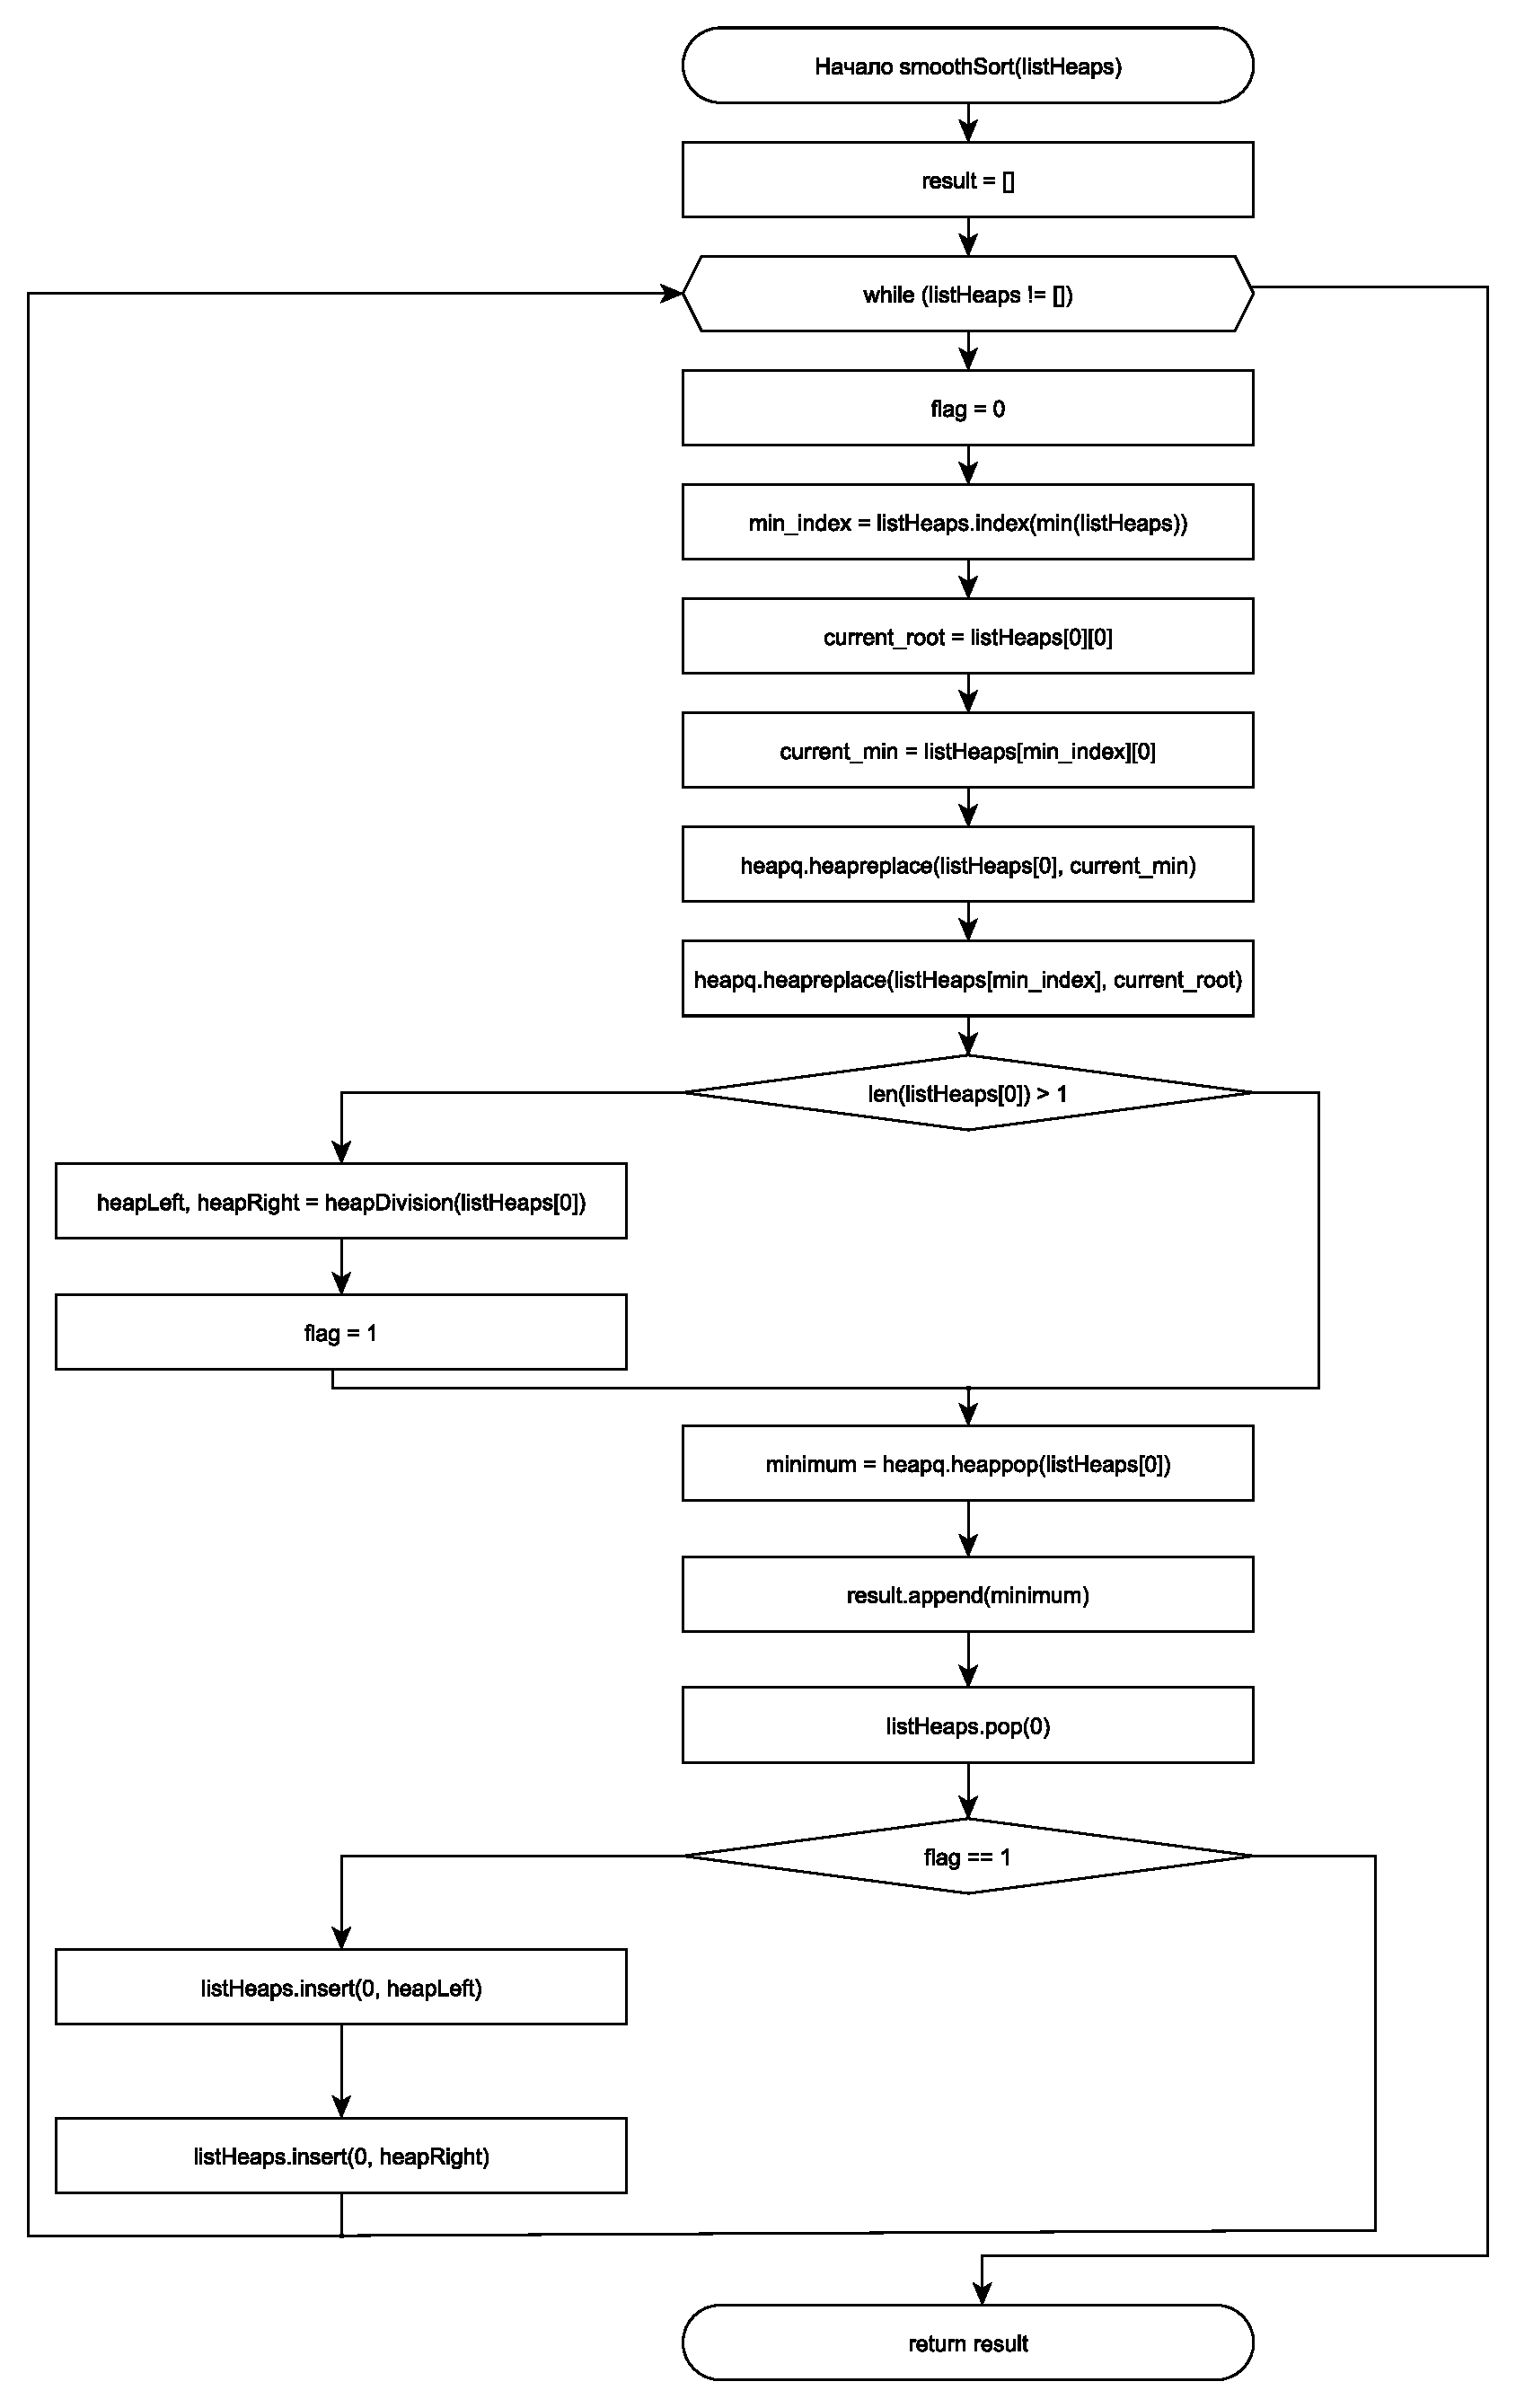
\includegraphics[width=\linewidth]{3.pdf}
	\caption{Зависимость средних значений от параметров}
	\label{graph2.7}
\end{figure}

Наборы параметров, при которых алгоритм ведёт себя стабильно:

\begin{table}[ht]
	\caption{Наборы параметров при стабильном результате}
	\begin{tabular}{|l|c|c|c|c|}
		\hline
		Набор & $\alpha$ & $\beta$ & ρ\\
		\hline
		\hline
		1 & 0 & 1 & 0.4 \\
		\hline
		2 & 1 & 0 & 0.8 \\
		\hline
	\end{tabular}
	\label{tab:tabular}
\end{table}

Наборы параметров, при которых алгоритм постепенно увеличивает длину найденного пути:

\begin{table}[ht]
	\caption{Наборы параметров при увеличении длины пути}
	\begin{tabular}{|l|c|c|c|c|}
		\hline
		Номер набора & $\alpha$ & $\beta$ & ρ\\
		\hline
		\hline
		1 & 0.2 & 0.8 & 0.2 \\
		\hline
		2 & 0.2 & 0.8 & 0.4 \\
		\hline
		3 & 1 & 0 & 0.6 \\
		\hline
	\end{tabular}
	\label{tab:tabular}
\end{table}

Наборы параметров, при которых алгоритм позволяет постепенно снижать длину найденного пути:

\begin{table}[ht]
	\caption{Наборы параметров при уменьшении длины пути}
	\begin{tabular}{|l|c|c|c|c|}
		\hline
		Номер набора & $\alpha$ & $\beta$ & ρ\\
		\hline
		\hline
		1 & 0 & 1 & 0 \\
		\hline
		2 & 0.2 & 0.8 & 1 \\
		\hline
		3 & 0.4 & 0.6 & 0 \\
		\hline
		4 & 0.4 & 0.6 & 1 \\
		\hline
		5 & 0.6 & 0.4 & 0 \\
		\hline
		6 & 0.8 & 0.2 & 1 \\
		\hline
	\end{tabular}
	\label{tab:tabular}
\end{table}

Набор параметров, рассматриваемых в гипотезе, заявленной в аналитическом разделе ($\alpha = 0.5, \beta = 0.5, ρ = 0.5$), при любом времени жизни колонии из рассматриваемого промежутка (от 1 до 10000) даёт минимальный путь из находимых муравьиным алгоритмом для данного примера, то есть 17. Результат остаётся аналогичным и в том случае, если при том же значении коэффициента испарения феромона параметры $\alpha = [0.4..0.5], \beta = [0.5..0.6]$.

\subsection{Сравнительный анализ на материале экспериментальных данных} 

В результате экспериментов подтвердилось то, что оптимальной является ситуация, когда $\alpha = 0.5, \beta = 0.5, ρ = 0.5$. Если параметры $\alpha$ и $\beta$ позволяли изменить их в противоположные стороны вплоть до $\Delta0.1$ относительно уравновешенного значения, то параметр ρ увеличивал найденную длину пути даже при изменении на 10\% в любую из сторон. 

Стабильное изменение результатов работы (в том числе, постоянный результат при различных значениях времени жизни из выборки) муравьиной колонии на неориентированном графе сопровождалось тем, что параметры начинали вырождаться.

 \clearpage
\addcontentsline{toc}{section}{Заключение}

\begin{center}
Заключение
\end{center}

В результате выполнения лабораторной работы была изучены задача коммивояжёра и способы её решения путём использования алгоритмов природных вычислений, получены навыки реализации муравьиного алгоритма, проведена его параметризация. Аналитическая параметризация, приведённая в конструкторском разделе, была подкреплена экспериментами. Было выявлено, что наилучший результат муравьиный алгоритм получает при $\alpha = 0.5, \beta = 0.5, ρ = 0.5$. Для коэффициента испарения феромона критичным оказалось даже изменение на 10\%. Параметры $\alpha$ и $\beta$ можно изменить до 10\% от этих значений при преобладании коэффициента $\beta$ (то есть 0.4 и 0.6 соответственно) без потери результата. В случае достижения параметрами граничных значений муравьиный алгоритм вырождается. Если $\alpha = 0$, то алгоритм становится жадным, а в противоположном случае перестаёт зависеть от расположения городов и начинает работать случайным образом. Если $ρ = 0$, то всё сведётся к жадному алгоритму, а если $ρ = 1$, то теряется зависимость от опыта предыдущих поколений колонии.

 \clearpage
\addcontentsline{toc}{section}{Список использованных источников}
\begin{thebibliography}{00} % Список литературы
\bibliographystyle{ugost2008}
\bibitem{TSP}
Задача коммивояжера - метод ветвей и границ. -- URL: $http://galyautdinov.ru/post/zadacha-kommivoyazhera$
\bibitem{AntAlg}
Штовба С. Д. Муравьиные алгоритмы, Exponenta Pro. Математика в приложениях. 2004. № 4
\bibitem{ACS}
M. Dorigo \& L. M. Gambardella, 1997. «Ant Colony System: A Cooperative Learning Approach to the Traveling Salesman Problem». IEEE Transactions on Evolutionary Computation, 1 (1): 53-66.
\bibitem{RECA}
М.В.Ульянов. Ресурсно-эффективные компьютерные алгоритмы $//$ 2007. - Раздел III. - Глава 7. - С.195-206.
\end{thebibliography}
\end{document}